%!TEX root = /home/renaud/Documents/EPL/tfe/latex/tfe.tex
\chapter{The "overturner" model}
\section{Mathematical model}
\subsection{An idealised velocity field}
We developp here the idealized representation of the meridian circulation in the Atlantic ocean that will be studied in the next chapters. \textcolor{red}{ici : développement mathématique. Plus loin on donne des valeurs aux paramètres avec un "physical insight"}. We consider a rectangular domain in the $(y,z)$-coordinate system. The coordinate $y$ is associated to the latitude with $\hat{\b{e}}_y$ pointing towards the North, and $z$ is associated to the depth with $\hat{\b{e}}_z$ pointing upwards. The domain $\Omega$ is delimited by
\begin{equation} 
	0 \le y \le L,\quad 0 \le z \le H,
\end{equation}
where $L$ and $H$ are positive constants. The ocean surface is thus located at $z = H$ while $z = 0$ stands for the deep-ocean. The South and North boundaries are respectively given by $y = 0$ and $y = L$. We aim at defining a stationnary velocity field $\b u(y,z) = (v(y,z),\, w(y,z))$ that would roughly reproduce the main qualitative features of the meridian circulation in the Atlantic ocean. The continuity equation reads
\begin{equation} \label{eq:continuity}
	\frac{\partial \rho}{\partial t} + \nabla \cdot (\rho \b u) = 0,
\end{equation}
where $\rho$ is the density of the seawater mixture. We note $\partial \Omega$ its boundary. We simplify this equation by making the very common \textit{Boussinesq appromation} : in the aquatic environment, water is, by far, the dominant constituent. The density of seawater is thus close to that of pure water, $\rho_w$. The latter depends on the temperature and pressure, but the variations are often very small.Let $\bar{\rho}$ and $\Delta\rho$ be appropriate reference values of the density and the order of magnitude of its variation. The key assumption in the \textit{Boussinesq approximation} is that
\begin{equation} \label{eq:bouss_hyp}
	\frac{\Delta \rho}{\bar{\rho}} \ll 1.
\end{equation}
To assess the impact of this assumption on the continuity equation, we consider its dimensionless form. Let $U$, $T$ and $X$ be relevant velocity-, time- and space-scales. This allows to introduce the following dimensionless variables, denoted by primes :
\begin{equation}
	\rho' = \frac{\rho - \bar{\rho}}{\Delta \rho}, \quad \b u' = \frac{\b u}{U}, \quad t' = \frac{t}{T}, \quad \mbox{and} \quad \b x' = \frac{\b x}{X},
\end{equation}
where $\b x = (y,z)$. The dimensionless version of the continuity equation \eqref{eq:continuity} reads then: 
\begin{equation}
	\frac{\Delta \rho}{T}\frac{\partial \rho'}{\partial t'} + \frac{U\Delta \rho}{X}\b u' \cdot \nabla' \rho' + \frac{U(\bar{\rho}+ \rho' \Delta \rho)}{X}\nabla' \cdot \b u' = 0.
\end{equation}
Multiplying both sides by $X/(U\bar{\rho})$ yields :
\begin{equation}
	\frac{X}{UT}\frac{\Delta \rho}{\bar{\rho}}\frac{\partial \rho'}{\partial t'} + \frac{\Delta \rho}{\bar{\rho}}\b u' \cdot \nabla' \rho' + \left(1+\frac{\Delta \rho}{\bar{\rho}}\rho'\right)\nabla' \cdot \b u' = 0.
\end{equation}
By taking \eqref{eq:bouss_hyp} into account, this equation simplifies to $\nabla' \cdot \b u' = 0$, or equivalently in dimensional variables $\nabla \cdot \b u = 0$. For our particular problem, this amounts to
\begin{equation}
	\frac{\partial v}{\partial y} + \frac{\partial w}{\partial z} = 0.
\end{equation}
No-through boundary conditions are imposed at the boundaries of the domain, which implies that $\b u(y,z) \cdot \hat{\b{n}} = 0$ everywhere on $\partial \Omega$ (where $\hat{\b{n}}$ is the outwards unit normal at the boundary), or equivalently :
\begin{equation} \label{eq:overturnerBC}
	v(0,z) = 0, \quad v(L,z) = 0, \quad w(y,0) = 0 \quad \mbox{and} \quad w(y,H) = 0.
\end{equation}
\textcolor{red}{Blahblah à mettre en relation avec ce qu'on doit dire plus tôt sur les modèles 2D de l'océan Atlantique,... Éventuellement s'inspirer de Timmermans mais attention quand même...}

Furthermore, since the relation $\nabla \cdot (\nabla \times \b a) = 0$ holds true for any 3-dimensional potential vector $\b a(x,y,z)$ whose second partial derivatives are continuous,\footnote{The proof is quite straightforward :
	\begin{align*}
		\nabla \cdot (\nabla \times \b a(x,y,z)) &= \nabla \cdot \left[\left(\frac{\partial a_z}{\partial y}-\frac{\partial a_y}{\partial z}\right)\ex + \left(\frac{\partial a_x}{\partial z}-\frac{\partial a_z}{\partial x}\right)\ey + \left(\frac{\partial a_y}{\partial x}-\frac{\partial a_x}{\partial y}\right)\ez \right]\\
		&= \frac{\partial^2 a_z}{\partial x \partial y} - \frac{\partial^2 a_y}{\partial x \partial z} + \frac{\partial^2 a_x}{\partial y \partial z} - \frac{\partial^2 a_z}{\partial y \partial x} + \frac{\partial^2 a_y}{\partial z \partial x} - \frac{\partial^2 a_x}{\partial z \partial y}\\
		&= 0.  
	\end{align*}
	Here, we have assumed that $\b a(x,y,z)$ is sufficiently smooth, or more precesily that the second partial derivatives of $a_x$, $a_y$ and $a_z$ are continuous. This allows to use \textit{Schwarz's theorem} which states that in that case, the second partial derivatives are symmetric.
} 
we can choose a relevant $\b a(x,y,z) = (a_x(x,y,z),\,a_y(x,y,z),\,a_z(x,y,z))$ with $a_x$, $a_y$ and $a_z$ of class $\C^2$ and impose that 
\begin{equation} \label{eq:stream3d}
	\b u = \begin{pmatrix} u \\ v \\ w \end{pmatrix} = - \nabla \times \b a = - \begin{pmatrix} \frac{\partial a_z}{\partial y}-\frac{\partial a_y}{\partial z}\\[.1 cm]
													\frac{\partial a_x}{\partial z}-\frac{\partial a_z}{\partial x}\\[.1 cm]
													\frac{\partial a_y}{\partial x}-\frac{\partial a_x}{\partial y}
									\end{pmatrix}.
\end{equation}
This ensures that $\b u$ satisfies the continuity equation. Here, we consider a 2-dimensional flow in the plane $(\ey,\ez)$. Hence $u = 0$ and $\partial \cdot/\partial x = 0$. The relation \eqref{eq:stream3d} becomes 
\begin{equation}
	\b u = \begin{pmatrix} 0 \\ v \\ w \end{pmatrix} = - \nabla \times \b a = \begin{pmatrix} 0\\ - \frac{\partial a_x}{\partial z}\\[.1 cm] \frac{\partial a_x}{\partial y} \end{pmatrix},
\end{equation}
where only the component $a_x$ is needed to describe $\b u$. Hence, the velocity field of a flow in the plane is described by a scalar quantity, the so-called \textit{streamfunction}, generally noted $\psi$. The potential vector $\b a$ is thus of the form $\b a(y,z) = (\psi(y,z),\, 0,\, 0)$, and the meridional and vertical components of the velocity vector are given by :
\begin{equation} \label{eq:u-psi}
	v = -\frac{\partial \psi}{\partial z}, \quad w = \frac{\partial \psi}{\partial y}.
\end{equation}
Note that adding any constant to $\psi$ leaves the velocity vector unchanged. This adds some freedom to the choice of $\psi$. The idea is now to propose a reasonable streamfunction. Then, deriving the velocity components from that streamfunction will ensure that the continuity equation is satisfied. In order to derive a streamfunction that is relevant to our problem, we need to get some physical intuition about the streamfunction. To this end, two fundamental properties of the streamfunction are rederived in the frame below. 

%--------------------------------------STREAMFUNCTION---------------------------------------------%
\begin{tcolorbox}[title=Some properties of the streamfunction]
First, notice that assuming that $\psi \in \C^2$ implies straightforwardly that $\rm d\psi = (\partial \psi/\partial y)\rm dy + (\partial \psi/\partial z) \rm dz$ is an \textit{exact differential} since by Schwarz's theorem
\begin{equation}
	\frac{\partial^2 \psi}{\partial y \partial z} = \frac{\partial^2 \psi}{\partial z \partial y}.
\end{equation}
Thus,
\begin{equation}
\int_{\b x_1}^{\b x_2} \rm d\psi = \psi(y_2,z_2) - \psi(y_1,z_1)	
\end{equation}
is path-independant. 

An important property of the streamfunction in two dimensions is that the curves along which $\psi$ is constant are exactly the \textit{streamlines} of the flow, namely the family of curves that are instantaneously tangent to the velocity vector. To show that, let such a curve be parametrized by $s \mapsto \b x_S(s) = (y_S(s),z_S(s))$. The fact that $\psi$ is constant along that curve implies that $\rm d\psi_S = (\partial \psi/\partial y)\rm dy_S + (\partial \psi/\partial z) \rm dz_S = \nabla \psi \cdot \rm d \b x_S = 0$. This shows that vector $\nabla \psi$ is normal to the curve $\b x_S(s)$. Hence, showing that $\b x_S(s)$ is everywhere tangent to $\b u$ is equivalent to showing that $\b u \cdot \nabla \psi = 0$ everywhere. The latter is straightforward using relation \eqref{eq:u-psi} :
\begin{equation}
	\b u \cdot \nabla \psi = -\frac{\partial \psi}{\partial z}\frac{\partial \psi}{\partial y} + \frac{\partial \psi}{\partial y}\frac{\partial \psi}{\partial z} = 0,
\end{equation}
which concludes the proof.

Now we show another interesting property of the streamlines, namely that the \textit{volume flow rate} between two streamlines of values $\psi_1$ and $\psi_2$ is equal to the difference of those streamlines, $\psi_1 - \psi_2$. To show that, consider two infinitely close points $\b x_1 = (y_1,\, z_1)$ and $\b x_1 + \rm d \b x = (y_1 + \rm dy,\, z_1 + \rm dz)$. At those points, the streamfunction has values $\psi(y_1,z_1) = \psi_1$ and $\psi(y_1+\rm dy,z_1 + \rm dz) = \psi_1 + \rm d\psi$. Let us now consider the volume flow rate $\rm dq$ accross the infinitesimal segment $[\b x_1,\, \b x_1 + \rm d \b x]$, positive in the right-hand side direction of the segment if the latter is directed from $\b x_1$ to $\b x_1 + \rm d \b x$. It is equal to $\b u \cdot \hat{\b{n}}$, where $\hat{\b{n}} = (\rm dz,\,-\rm dy)$ is the unit normal to the segment, oriented in the right-hand side direction. Hence, $\rm dq = v \rm dz - w \rm dy$, which, using relation \eqref{eq:u-psi}, amounts to
\begin{equation}
	\rm dq = - \rm d\psi.
\end{equation}
Now, consider any two points $\b x_1 = (y_1, z_1)$ and $\b x_2 = (y_2, z_2)$ in the (connected) domain. The volume flow rate $q_{1 \rightarrow 2}$ accross any curve $\gamma_{1 \rightarrow 2}$ connecting $\b x_1$ to $\b x_2$, positive in the right-hand side direction of the directed segment $[\b x_1,\, \b x_2]$ is
\begin{equation}
	q_{1 \rightarrow 2} = \int_{\gamma_{1 \rightarrow 2}} \rm dq = \int_{\b x_1}^{\b x_2} (-\rm d\psi) = \psi(y_1,z_1) - \psi(y_2,z_2), 	
\end{equation} 
where $\int_{\gamma_{1 \rightarrow 2}}$ is the line integral along a curve connecting $\b x_1$ to $\b x_2$, afterwards noted $\int_{\b x_1}^{\b x_2}$ to emphasize the fact that it does not depend on the integration path, since $\rm d\psi$ is an exact differential.
\end{tcolorbox}
%----------------------------------------END STREAMFUNCTIONS-------------------------------------------%
Now we are able to derive a relevant streamfunction. In particular, $\psi$ must be such that the boundary conditions \eqref{eq:overturnerBC} are satisfied. Those conditions state that $\b u$ must be tangent to the boundary everywhere on $\partial \Omega$, which precisely amounts to require that $\psi$ is constant on $\partial \Omega$. Without loss of generality, we can choose this constant to be zero. Hence, we require that 
\begin{equation}
	\psi(0,z) = 0, \quad \psi(L,z) = 0, \quad \psi(y,0) = 0 \quad \mbox{and} \quad \psi(y,H) = 0, \quad \mbox{for all $(y,z) \in \Omega$}.
\end{equation}
\textcolor{red}{Faire des liens avec chapitre précédent} In order to build an acceptable idealisation of the meridian circulation in the Atlantic ocean, \textit{Deleersnijder} proposes in his working paper \cite{deleersnijder2006overturner} to suppose that the meridian streamfunction has a unique extremum $\Psi$, which is a maximum, and that it reaches that maximum at the point of coordinates $(y_0,z_0)$, located near the surface and the North boundary of the domain. It is important to recall that the second partial derivatives of $\psi$ must exist and be continuous for the above relations to hold.

Let $\xi_0 \in \mathbb{R}_0^+$, and let $\phi(\xi,\xi_0)$ be defined as
\begin{equation} \label{eq:phi}
	\phi(\xi,\xi_0) = \frac{\xi(2\xi_0-\xi)}{\xi_0^2},
\end{equation}
The derivative $\phi'(\xi,\xi_0)$ of $\phi$ with respect to $\xi$ is
\begin{equation}
	\phi'(\xi,\xi_0) = \frac{2(\xi_0-\xi)}{\xi_0^2}.
\end{equation}
An expression of the meridian streamfunction that satisfies the above constraints is then
\begin{equation} \label{eq:psi_overturner}
	\psi(y,z) = \Psi\left\{ 
		\begin{array}{lrr}
			\phi(y,y_0)\phi(z,z_0) & \mbox{if} & 0 \le y < y_0, \phantom{z_0}0 \le z < z_0,\\
			\phi(y,y_0)\phi(H-z,H-z_0) & \mbox{if} & 0 \le y < y_0, \phantom{0}z_0 < z \le H,\\
			\phi(L-y,L-y_0)\phi(H-z,H-z_0) & \mbox{if} & y_0 < y \le L, \phantom{0}z_0 < z \le H,\\
			\phi(L-y,L-y_0)\phi(z,z_0) & \mbox{if} & y_0 < y \le L, \phantom{z_0}0 \le z < z_0.
		\end{array}
	\right.
\end{equation}
As such, $\psi$ is undefined along the lines $y = y_0$ and $z = z_0$. We consider thus the continuous prolongation of $\psi$ at those points. Hence, 
\begin{equation} \label{eq:psi_y0}
	\psi(y_0,z) = \Psi\left\{ 
		\begin{array}{lrr}
			\phi(z,z_0) & \mbox{if} & 0 \le z < z_0,\\
			\phi(H-z,H-z_0) & \mbox{if} & z_0 < z \le H,\\
		\end{array}
	\right.
\end{equation}
\begin{equation} \label{eq:psi_z0}
	\psi(y,z_0) = \Psi\left\{ 
		\begin{array}{lrr}
			\phi(y,y_0) & \mbox{if} & 0 \le y < y_0,\\
			\phi(L-y,L-y_0) & \mbox{if} & y_0 < y \le L,\\
		\end{array}
	\right.
\end{equation}
and
\begin{equation}
	\psi(y_0,z_0) = \Psi.
\end{equation}

The meridian and vertical components of the velocity are then expressed as
\begin{equation} \label{eq:v_overturner}
	v(y,z) = \Psi\left\{ 
		\begin{array}{lrrr}
			- \phi(y,y_0)\phi'(z,z_0) & \mbox{if} & 0 \le y < y_0, & 0 \le z < z_0,\\
			\phi(y,y_0)\phi'(H-z,H-z_0) & \mbox{if} & 0 \le y < y_0, & z_0 < z \le H,\\
			\phi(L-y,L-y_0)\phi'(H-z,H-z_0) & \mbox{if} & y_0 < y \le L, & z_0 < z \le H,\\
			- \phi(L-y,L-y_0)\phi'(z,z_0) & \mbox{if} & y_0 < y \le L, & 0 \le z < z_0,\\
			- \phi'(z,z_0) & \mbox{if} & y = y_0, & 0 \le z < z_0,\\
			\phi'(H-z,H-z_0) & \mbox{if} & y = y_0, & z_0 < z \le H,\\
			0 & \mbox{if} &0 \le y \le L, & z = z_0.
		\end{array}
	\right.
\end{equation}
and
\begin{equation} \label{eq:w_overturner}
	w(y,z) = \Psi\left\{ 
		\begin{array}{lrrr}
			\phi'(y,y_0)\phi(z,z_0) & \mbox{if} & 0 \le y < y_0, & 0 \le z < z_0,\\
			\phi'(y,y_0)\phi(H-z,H-z_0) & \mbox{if} & 0 \le y < y_0, & z_0 < z \le H,\\
			- \phi'(L-y,L-y_0)\phi(H-z,H-z_0) & \mbox{if} & y_0 < y \le L, & z_0 < z \le H,\\
			- \phi'(L-y,L-y_0)\phi(z,z_0) & \mbox{if} & y_0 < y \le L, & 0 \le z < z_0,\\
			\phi'(y,y_0) & \mbox{if} & 0 \le y < y_0, & 0 \le z = z_0,\\
			- \phi'(L-y,L-y_0) & \mbox{if} & y_0 < y \le L, & z = z_0,\\
			0 & \mbox{if} & y = y_0. &
		\end{array}
	\right.
\end{equation}

\subsection{Estimation of the parameter values}
\textcolor{red}{Vérifier que c'est bien les valeurs finales}
The numerical values used here are based on personal communications with \textit{E. Deleersnijder}.
The model for the idealised meridian velocity field in the Atlantic ocean will be complete once we have assigned plausible values to the parameters. For this purpose, some physical insight is needed. First, the Atlantic ocean extends approximately from $50\degree$ South to $60\degree$ North, hence over $\frac{11}{18}\pi$ radians. With the radius of the Earth estimated to $6\,371$ km, we get that $L$ must be close to $(\frac{11}{18}\pi) (6\,371) = 12\, 231$ km. Moreover, the mean depth of the Atlantic ocean is about $4$ km. Hence, we choose $L = 12\,000$ km and $H = 4$ km. In virtue of the properties of the streamfunction, the maximum $\Psi = \psi(y_0,z_0)$ of the meridian streamfunction is equal to the volume flow rate accross any curve connecting $(y_0,z_0)$ to a point on the boundary of the domain: it is thus a measure of the intensity of the meridian circulation. With an estimated rate of deep convection in the Atlantic ocean of about $20$ Sv and a mean width of about $5\,000$ km, this yields $\Psi = 4$ $\rm{m^2/s}$. Finally, we use $y_0 = 11\,000$ km and $z_0 = 3.5$ km based on qualitative inspection of the meridian streamfunction graph. Characteristic values $V$ and $W$ of the meridional and vertical speed are, in virtue of relations \eqref{eq:u-psi} :
\begin{equation}\label{eq:VW}
	V = \frac{\Psi}{H} \quad \mbox{and} \quad W = \frac{\Psi}{L}.
\end{equation}
According to \textit{E. Deleersnijder} [personal communication], the characteristic time scale $T$ should be of the order of a few hundred years in order to be physically significant. It is expressed as
\begin{equation} \label{eq:T}
	T = \frac{L}{V} = \frac{H}{W} = \frac{LH}{\Psi} = 1.5\e{6} \mbox{ s} \approx 475.6 \mbox{ years},
\end{equation}
an acceptable value.

With those values of the parameters, the isolines of the adimensional streamfunction $\psi/\Psi$ are shown in figure \ref{fig:psi_overturner}, and the meridional and vertical components of the velocity field are illustrated in figure \ref{fig:vw_overturner}.
\begin{figure}[ht]
	\centering
	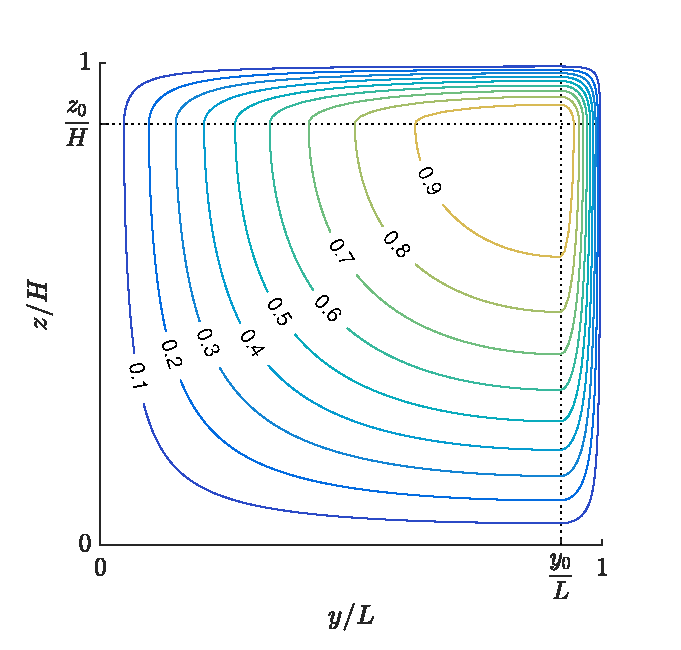
\includegraphics[width=.6\textwidth]{fig/overturner/psi.eps}
	\caption{Some isolines of the adimensional meridian streamfunction $\psi(y,z)/\Psi$, which are also streamlines of the idealised meridian circulation in the Atlantic ocean.}
	\label{fig:psi_overturner}
\end{figure}

\begin{figure}[ht]
	\centering
	\begin{subfigure}[t]{0.4\textwidth}
		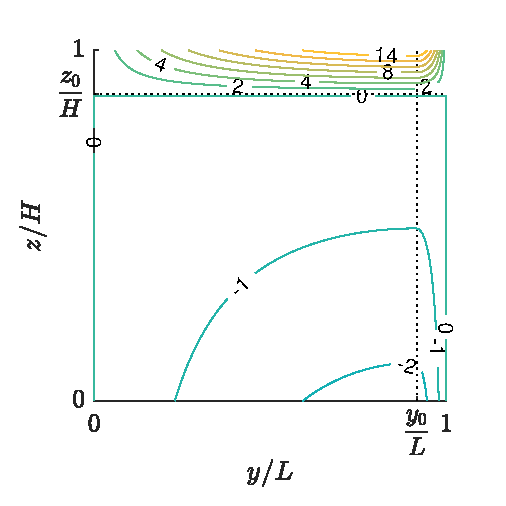
\includegraphics[width=\textwidth]{fig/overturner/V_samecaxis.eps}
		\caption{$v(y,z)$.}
		\label{fig:v_overturner}
	\end{subfigure}
	\begin{subfigure}[t]{0.4\textwidth}
		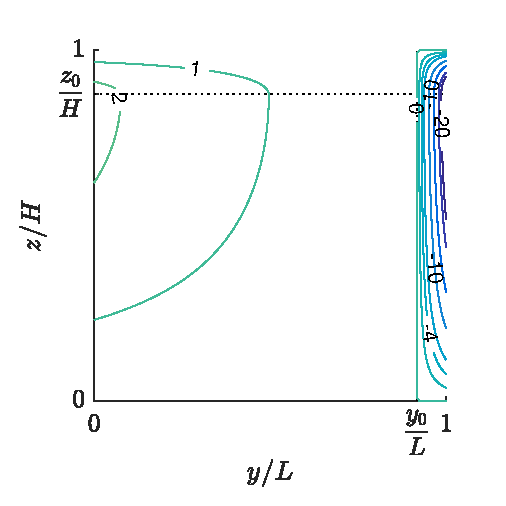
\includegraphics[width=\textwidth]{fig/overturner/W_samecaxis.eps}
		\caption{$w(y,z)$.}
		\label{fig:w_overturner}
	\end{subfigure}
	\begin{subfigure}[t]{0.1\textwidth}
		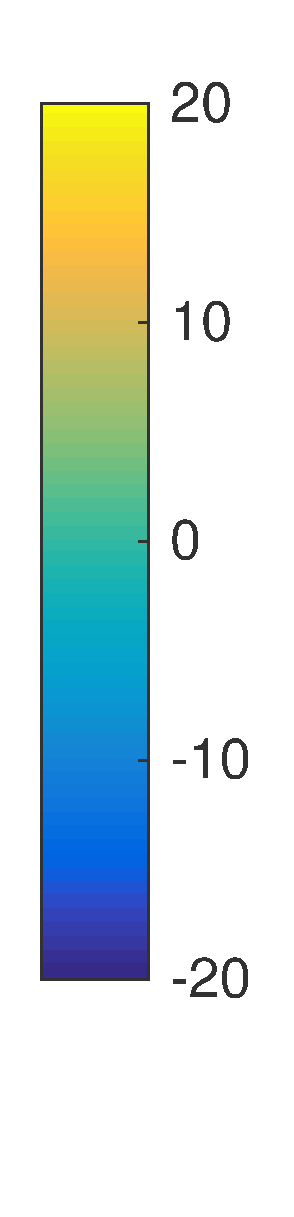
\includegraphics[height = 4\textwidth]{fig/overturner/colorbarVW.eps}
	\end{subfigure}
	\caption{Meridional and vertical components of the idealised velocity fields in the adimensional domain. Here, $y_0 = \frac{11}{12}L$ and $z_0 = \frac{7}{8}H$.}
	\label{fig:vw_overturner}
\end{figure}

\subsection{Injection of a passive tracer into the ocean}
The fate of a passive tracer injected at location $(y_*,z_*)$ into the idealised Atlantic ocean depicted previously can be described by a differential problem on that tracer's concentration. The tracer could be any passive tracer whose concentration in the athmosphere is negligible, for example a dye or a set of seawater particles initially located at $(y_*,z_*)$. The concentration of the tracer $C(t,y,z)$ in the ocean obeys the following partial differential equation :
\begin{equation}\label{eq:C_PDE_vec}
	\frac{\partial C}{\partial t} = -\nabla \cdot \left(\b uC - \b K \nabla C\right),
\end{equation}
where $\b K$ is the \textit{diffusivity tensor}. Without loss of generality, we can assume $\b K$ to be symmetric. This is essentially because the impact of the anti-symmetric part of $\b K$, if any, may be viewed as additional advection. More details may be found in appendix A of \cite{deleersnijder2001concept}. Of course, the symmetric tensor $\b K$ must then be positive-definite in order to represent truly diffusive processes, namely phenoma which tend, at any time and location, to homogenise the concentration of any constituent. For our problem, we consider that $\b K$ has the form
\begin{equation} \label{eq:K}
	\b K(y,z) = \begin{pmatrix} K_h & 0 \\ 0 & K_v(y,z) \end{pmatrix},
\end{equation}
where $K_h$ is a positive constant and
\begin{equation} \label{eq:Kv}
	K_v(y,z) = \left\{ 
		\begin{array}{lrrr}
			K_{v_1} & \mbox{if} & y_0 \le y \le L, & 0 \le z \le H,\\
			K_{v_2} & \mbox{if} & 0 \le y < y_0, & 0 \le z < z_0,\\
			K_{v_3} & \mbox{if} & 0 \le y < y_0, & z_0 \le z \le H,
		\end{array}
	\right.
\end{equation}
with $K_{v_1}$, $K_{v_2}$ and $K_{v_3}$ positive constants. In the framework of the idealised model of the meridian circulation in the Atlantic ocean, \textit{E. Deleersnijder} [personal communication] proposes the values $K_h = 10^3$ $\rm{m^2/s}$, $K_{v_1} = 10^{-1}$ $\rm{m^2/s}$, $K_{v_2} = 10^{-4}$ $\rm{m^2/s}$ and $K_{v_3} = 10^{-3}$ $\rm{m^2/s}$. The relatively large value of $K_{v_1}$ allows to represent deep convection in the corresponding zone without having to implement a convective adjustment algorithm. The developped form of \eqref{eq:C_PDE_vec} is then
\begin{equation}\label{eq:C_PDE_dev}
	\frac{\partial C}{\partial t} = -\frac{\partial}{\partial y}\left(vC - K_h\frac{\partial C}{\partial y}\right) -\frac{\partial}{\partial z}\left(wC - K_v(y,z)\frac{\partial C}{\partial z}\right).
\end{equation}
No-flux conditions are imposed at the boundaries \textcolor{red}{vérifier/discuter le flux nul à la surface}
\begin{equation}\label{eq:C_PDE_BC}
	\left. K_h\frac{\partial C}{\partial y} \right|_{y=0} = 0, \quad  \left. K_h\frac{\partial C}{\partial y} \right|_{y=L} = 0, \quad \left. K_v\frac{\partial C}{\partial z} \right|_{z=0} = 0, \quad \mbox{and} \quad \left. K_v\frac{\partial C}{\partial z} \right|_{z=H} = 0.
\end{equation}
The initial condition is
\begin{equation} \label{eq:C_PDE_CI}
	C(0,y,z) = \delta(y-y_*)\delta(z-z_*),
\end{equation}
where $\delta$ is the Dirac delta function, such that
\begin{equation}
	\int_0^L \int_0^H C(0,y,z) \rm dy \rm dz = 1.
\end{equation}

In order to get a formulation of the problem using as few independant parameters as possible, it is interesting to consider the adimensional formulation. Such a scaling is particularly interesting for sensitivity analysis. The adimensional independant variables are
\begin{equation}
	t' = \frac{t}{T} = \frac{t\Psi}{LH}, \quad y' = \frac{y}{L} \quad \mbox{and} \quad z' = \frac{z}{H},   	
\end{equation}
where $T$ is the time scale introduced in \eqref{eq:T}. The adimensional hydrodynamic variables are:
\begin{equation}
	\psi' = \frac{\psi}{\Psi}, \quad v' = \frac{v}{V} = \frac{vH}{\Psi}, \quad \mbox{and} \quad w' = \frac{w}{W} = \frac{wL}{\Psi},
\end{equation}
where $V$ and $W$ are the velocity scales introduced in \eqref{eq:VW}. The adimensional concentration is
\begin{equation}
	C' = \frac{C}{C_r}, 	
\end{equation}
where $C_r$ is a characteristic value of the concentration. We will see shortly that there is no needed to assign a particular value to $C_r$. The adimensional form of equation \eqref{eq:C_PDE_dev} is then
\begin{equation}\label{eq:PDE_adim}
	\frac{\partial C'}{\partial t'} = -\frac{\partial}{\partial y'}\left(v'C' - \frac{1}{Pe_h}\frac{\partial C'}{\partial y'}\right) -\frac{\partial}{\partial z'}\left(w'C' - \frac{1}{Pe_v(y,z)}\frac{\partial C'}{\partial z'}\right),
\end{equation}
where
\begin{equation}
	Pe_h = \frac{\Psi L}{K_h H} \quad \mbox{and} \quad Pe_v(y,z) = \frac{\Psi H}{K_v(y,z)L}
\end{equation}
are the horizontal and vertical Péclet numbers. They correspond to the ratio between the characteristic advective and diffusive velocity scales. Indeed, the horizontal and vertical diffusive velocity scales $V_{d}$ and $W_{d}$ are 
\begin{equation}
	V_{d} = \frac{K_h}{L} \quad \mbox{and} \quad W_{d}(y,z) = \frac{K_v(y,z)}{H}.
\end{equation}
There are three different vertical diffusive velocity scale depending on which zone of the ocean we consider \textcolor{red}{Donner des noms aux zones dans le chap 1 : 1 = ?, 2 = "Deep convection" et 3 = "surface flow"}. The advective velocity scales $V$ and $W$ have already been introduced in \eqref{eq:VW}. The Péclet numbers may then be rewritten as
\begin{equation}
	Pe_h = \frac{V}{V_{d}} = 12, 
\end{equation}
and
\begin{equation}
	Pe_{v}(y,z) =  \frac{W}{W_{d}(y,z)}=  \left\{
	\begin{array}{lrrr}
			Pe_{v_1} = 1.33\e{-2} & \mbox{if} & y_0 \le y \le L, & 0 \le z \le H,\\
			Pe_{v_2} = 13.3 & \mbox{if} & 0 \le y < y_0, & 0 \le z < z_0,\\
			Pe_{v_3} = 1.33 & \mbox{if} & 0 \le y < y_0, & z_0 \le z \le H.
	\end{array}
	\right.
\end{equation}
This shows that the advective and diffusive processes are of equal importance in the dynamics of our model, excepted in the zone of deep convection where the vertical diffusion dominates the vertical convection. This is because we have chosen to represent deep convection via a heavy vertical mixing in that zone. 